
\documentclass[twoside, twocolumn]{article}

\usepackage[sc]{mathpazo} % Use the Palatino font
\usepackage[T1]{fontenc} % Use 8-bit encoding that has 256 glyphs
\linespread{1.05} % Line spacing - Palatino needs more space between lines
\usepackage{microtype} % Slightly tweak font spacing for aesthetics

\usepackage[english]{babel} % Language hyphenation and typographical rules

\usepackage[hmarginratio = 1:1,
top 		 = 32mm,
columnsep    = 20pt]{geometry} % Document margins
\usepackage[hang, 
small,
labelfont = bf,
up,
textfont  = it,
up]{caption} 									% Custom captions under/above floats in tables or figures

\usepackage{booktabs} 										% Horizontal rules in tables

\usepackage{lettrine}										% The lettrine is the first enlarged letter at the beginning of the text
\usepackage{appendix}
\usepackage{enumitem} 										% Customized lists
\setlist[itemize]{noitemsep} 								% Make itemize lists more compact

\usepackage{abstract} 										% Allows abstract customization
\renewcommand{\abstractnamefont}{\normalfont\bfseries} 		% Set the "Abstract" text to bold
\renewcommand{\abstracttextfont}{\normalfont\small\itshape} % Set the abstract itself to small italic text

\usepackage{titlesec} 										% Allows customization of titles
\renewcommand\thesection{\Roman{section}} 					% Roman numerals for the sections
\renewcommand\thesubsection{\roman{subsection}}				% roman numerals for subsections

\titleformat{\section}[block]{\large\scshape\centering}{\thesection.}{1em}{} % Change the look of the section titles
\titleformat{\subsection}[block]{\large}{\thesubsection.}{1em}{} % Change the look of the section titles

\usepackage{fancyhdr} % Headers and footers
\pagestyle{fancy}	  % All pages have headers and footers
\fancyhead{} 		  % Blank out the default header
\fancyfoot{} 		  % Blank out the default footer
\fancyhead[C]{change this - \today - Master thesis} % Custom header text
\fancyfoot[RO,LE]{\thepage} % Custom footer text

\usepackage{titling} % Customizing the title section
\usepackage{hyperref} % For hyperlinks in the PDF


% custom
\usepackage{amsmath}
\usepackage[backend=biber, bibencoding=utf8, style=nature, url=false]{biblatex}
\addbibresource{/home/casper/biblatex/computational_science.bib}
\usepackage{graphicx}
\usepackage{float}
%----------------------------------------------------------------------------------------
%	TITLE SECTION
%----------------------------------------------------------------------------------------

\setlength{\droptitle}{-4\baselineskip} % Move the title up

\pretitle{\begin{center}\Huge\bfseries} % Article title formatting
	\posttitle{\end{center}} % Article title closing formatting
\title{Climbing the ladder of causation} % Article title
\author{%
	\textsc{Casper van Elteren} \\[1ex] % Your name
	\normalsize Radboud University \\ % Your institution
	\normalsize \href{mailto:caspervanelteren@gmail.com}{caspervanelteren@gmail.com} % Your email address
	%\and % Uncomment if 2 authors are required, duplicate these 4 lines if more
	%\textsc{Jane Smith}\thanks{Corresponding author} \\[1ex] % Second author's name
	%\normalsize University of Utah \\ % Second author's institution
	%\normalsize \href{mailto:jane@smith.com}{jane@smith.com} % Second author's email address
}
\date{\today} % Leave empty to omit a date
\renewcommand{\maketitlehookd}{%
	\begin{abstract}
		\noindent One of the most central questions in network science is: which nodes are most important? Often this is answered using topological properties such as high connectedness or centrality in the network. However it is unclear whether topological connectedness translates directly to dynamical influence. Here we show that topological features such as network centrality or connectedness are actually poor predictors of the dynamical influence of a node on the rest of the network. We simulate the kinetic Ising spin model with weighted edges on generated and real weighted networks, including a psychological symptom network. Dynamical importance of a node is predicted by the characteristic time of decay of information about its state variable, and validated by simulating perturbations to node states. One of our main findings is that the most dynamically  influential nodes are usually not the most well-connected or central nodes. This implies that the common assumption of topologically central or well-connected nodes being also dynamically important is actually false, and we cannot abstract away the dynamics from a network before analyzing it.
	\end{abstract}
}



\date{\today}
\begin{document}
	
	\maketitle
	\thispagestyle{empty}
	

%	\section*{First bit}
%	If you want to ramp your text straight onto the title page, start the text at 
%	something that does not cause a page break, like a section.  Here's a handy 
%	place to introduce some of your woofy conventions, like quotes in equations.
	\section*{Introduction}
	% causal explanations
	% emergent behavior
	% topology centric approach
	% we willen meest impactvol node uitharden; is degene met de hoogste idt ook de node met meest impact? vorig onderzoek neit gedaan
%	 hoe is de ranking na nudge?
	One of the principle aims of science is to provide causal explanation to (natural) phenomena\cite{Woodward2005, Pearl2000}. For example, we wish to understand why healthy cells can transform into cancerous cells, how populations of neurons produce cognition, what causes a financial market to crash,  or how social interaction influences opinion consensus. These systems are typically characterized by many dynamical variables, non-equilibrium, non-linear, and time-dependent behavior, defying analysis by most of our current theories and tools. At the same time, exactly these systems are vitally important to the functioning of our bodies, society, and environment. Their resistance to reductionistic analysis has earned them the qualification of `complex (adaptive) systems' and spawned the cutting edge field of complexity science aiming to understand the inner-mechanism of these systems\cite{Mitchell1998, Sayama2015}. 
	
	Obtaining causal explanations is a multi-step process. Pearl identified three levels of causation\cite{Pearl2018}. The first step in understanding any problem is mapping regularities in the environment. This level is where science starts and where it is the state of the art for the many supervised machine learning methods specifically neural networks including deep learning. The second level entails predicting the effects of deliberate alterations of the environment. It focuses on `what-if' scenarios, e.g. what will happen if we change the environment. It is important to emphasize that the first level will never be enough for causal explanations. No matter how large the dataset is, passive observation will only yield correlative associations where cause and effect cannot be disentangled.  The final step involves constructing theories surrounding `why' questions, e.g. questions such as `Was it $X$ that caused $Y$?' or `What if $X$ had not occured?'. That is, the final level op causation looks to the past and is able to integrate information above-and-beyond the second level. It allows for answering of counter-factuals through control and manipulation and is crucial for understanding the problems outlined above. 
	
	Reaching the final level of causation is not trivial however. Current available theories and algorithms for inferring the causal influence of dynamic variables are not readily applicable to complex systems. Four major issues can be identified from literature. First, many theories and algorithms are developed using at least one of the following assumptions regarding system behavior, e.g. stationarity of system state, (local) linearity of dynamics\cite{Chen2017, Liu2016a}, time-independence of the interaction, and/or having reached equilibrium. Second, techniques differ in strength of intervention. Many techniques are based on the `overwhelming' control intervention \cite{Chen2017}, e.g. completely knocking out a gene from a cell's regulatory process, or replacing its signal altogether. Especially in complex systems such dramatic interventions may completely change the emergent system behavior or lead to undesirable side-effects and should therefore be avoided. 
	Third, identification of causally important parts of a system, i.e. dynamically important for the systemic behavior, has long been studied from the viewpoint of topology\cite{Harush2017a,Sikic2013,Cowan2012, Muldoon2016, Yan2017, Pequito2017}. This viewpoint is often based on concepts of `flow'; the more outward connections a node in a system has, the more opportunities it has for spreading its information. For example, (structural) control theory identifies sets of driver-nodes based on their coverage of the edges in a graph. However, it is well-know that topology interacts with dynamics\cite{Cowan2012, Harush2017a, Gates2016}. A recent study showed that the same static topoloy dictated by different dynamics yield different node influence \cite{Harush2017a}. This means that as the dynamic on a network structure changes, so does the dynamic importance of that node. Therefore, identifying possible causal driver-nodes cannot reliably be determined based on topology measures alone. Additionally, obtaining control using a topology based method may not be feasible on real-world network, e.g. it may require extraneous long time \cite{Pequito2017} or require abnormally large interventions\cite{Cowan2012, Yan2012}.
	Lastly, the asymmetry of causal influence is not always accounted for. The rules of algebra allow to write relations between variables in a variety of syntatic forms. To illustrate consider Newton's second law of motion $f = m a$. This equation can be written in different ways, however it is common to think that force \textit{causes} acceleration - not that acceleration causes force. The causal asymmetry of cause and effect cannot be inferred from a symmetrical equation. This lack of asymmetry is a problem for `unification' accounts in mathematics and physics where the goal is to find one formula that could explain or account for different natural phenomena such as quantum particle motion, gravity. Providing causal explanations inherently requires scientists to embed the analysis in an asymmetrical environment using control and manipulation. 
	
	In this thesis, we aim to further develop and validate a novel algorithm for inferring the primary causal driver nodes of a complex system\cite{Quax2013}. Previous research showed that it was not the high-degree nodes in scale-free artificial networks that were dynamically most important, rather the intermediately-connected nodes were proofed to be dynamically more salient. Here, we specifically focus on determining if topological features are a good predictor for the primary driver-node in a real-world signed network.  Additionally, the aim is to expand the proposed methods through a framework of control and manipulation(\ref{sec:methods}). 
	
	At its core the method consists of information-theoretic measures, specifically a time-delayed version of Shannon mutual information (MI)\cite{Cover2005} which are computed based on cross-section of time-series of each dynamic variable in the system with the entire system. Information theoretical methods have the advantage of being suitable for non-equilibrium systems, and non-linear,  time-dependent interactions. Additionally, they can be readily applied to different data-types such as categorical, discrete and continuous data. Furthermore, the technique will be a good predictor for specifically small interventions and not overwhelming interventions, making it suitable for sensitive control of complex systems while staying as close as possible to their natural functioning. 
	
	Similar approaches have been developed using other information theoretical based approaches such as transfer entropy \cite{Eichler2006}, conditional MI \cite{Wibral2014}, relative entropy\cite{AY2008} or information bottleneck\cite{Tishby2000}. However, these methods are not suitable for two reasons. Firstly, the  question that these techniques attempt tot answer is qualitatively different from our proposed measure. Their main aim is to reconstruct the complete network of causal interactions by evaluating the (short-term) causal influence between every pair of nodes. In contrast, the emphasis here is on finding out whether a give-node has a long-term causal effect on the entire system - \textit{regardless of where in the system this effect resides}. Second, they are ultimately based on the conditional MI measure which is known to either overestimate or underestimate the influence of so-called synergistic and redundant information\cite{James2016a}. The used methods here circumvents this issue by using only the non-conditional MI measure which does not have this problem. This has the disad\left( vantage that only a handful (independent) driver-nodes can be identified instead of the full causal network. Regardless, this body of work will already provide essential innovation towards the management of complex systems and possible research avenue for climbing the ladder of causation.
	
	
	
		
	
	\section{Material and Methods} \label{sec:methods}
	\subsection{Information decay time}
	
	The goal is to identify driver-nodes in the system. A driver-node is defined as a node that has the most dynamic impact on the system over time, i.e. it will `drive' the system. Here we identify the most impactful node  not based on topological features, but rather on dynamic properties by using concepts from information theory \cite{Quax2013}.
	
	
	A system $G = (V, E, D)$ is defined as set of nodes or vertices $v_1, v_2, \cdots, v_k \in V$ and edges $(v_i, v_j)\in E$ between which interactions can take place. Each node in the system is dictated by dynamics $D$. The state of node $v_i$ at time $t$ is defined as $v_i(t)$ and the state of the system (or `snapshot') is the collection of node states $V^t = \{v_1(t), v_2(t), \cdots v_k(t)\}$. Each node in the network chooses its next state based on the current state and the state of each of its nearest-neighbors, i.e. node $v_i(t)$ chooses its next state $x$ with the conditional probability distribution $p(v_i(t+1) = x \vert h_i(t))$ where $h_i(t) = \{x: (v_i(t), x) \in E\}$ are the nearest-neighbors of node $i$. This is also known as a Markov-network or memory-less dynamics. 
	
	
	The dynamic importance of a node $v_i$ is quantified by the information decay time (IDT) \cite{Quax2013}. The IDT is the time $\delta$ it takes for the information about the state of node $s$ to disappear from the network state. Conversely, it is the time it takes for the network as a whole to forget a particular state of a single node. We quantify `forgetting' in terms of the decay of \textit{ bits of information} using a time-delayed Shannon mutual information. A bit of information is conceptualized as the minimum required yes-no questions to determine the outcome of a stochastic variable $X$ and is quantified using entropy\cite{Shannon1948}:
	
	\begin{equation}\label{entropy}
	H(X) = - \sum_x p(x) \log p(x)
	\end{equation}
	Please note that all $\log$ are base 2 in this paper. 
	Entropy is often conceptualized as the amount of `surprise' of a stochastic variable. To illustrate, consider a far coin. It requires exactly one yes-no question to determine the state of the coin after a flip, e.g. was the facing side heads or conversely tails? Hence, the fair coin can deliver 1 full bit of information. In contrast, if the coin was not fair, the conveyed information would be less because of the reduction in surprise\cite{Cover2005}. 
	
	Mutual information can be thought of as the reduction of uncertainty about one random variable given the knowledge of another random variable, i.e. $I(X;Y) = H(X) - H(X \vert Y)$ , where $H(X)$ and $H(X\vert Y)$ indicates the entropy and conditional entropy respectively. The conditional entropy is similar to the entropy except that it takes into  account the effect of a second variable, specifically how much uncertainty is left after taking into account another variable. High mutual information indicates a large reduction in uncertainty, and zero mutual information between two random variables means that the variables are independent. 
	
	\subsection{Defining information dissipation of a node}
	Up until now, we haven't addressed how we can ensure that the information of a node will be lost as a function of time. This can be ensured using the data processing inequality. This concept from information theory entails that the information content of a signal cannot be increased through physical operation in a Markov chain; information is generally lost, not gained when sent through a noisy channel, see \ref{app:dpi} for proof.
	
	At every time step every node can partially transmit its information to its nearest neighbors. In order to compute the IDT we will need a time-delayed mutual information which is defined as:
	\begin{equation} \label{eq:mi}
	\begin{aligned}
	I(s_i(t) ; S(0)) &= H(s_i(t)) - H(s_i(t) \vert S(0)) \\
	&= \sum_{s_i(t)=x}  \sum_{S(0) = X} P(x \vert X) \log \frac{P(x \vert X)}{P(x)}
	\end{aligned}
	\end{equation}
	The state $S(0) = X$ indicates a random state from the state space of the system, i.e. a specific `snapshot' or configuration of the system, and $s_i(t)$ indicates the state of node a node at some time $t$ from snapshot $S(0)$, please see \ref{sec:numerical}. 
	
	Here we consider Markovian networks in which each node determines its next state according to the Gibbs measure. The Gibbs measure describes how a unit changes its state subject to the combines potential of its interacting neighbors (see \ref{sec:model}). We define the IDT for node $s_i$ as :
	\begin{equation}
	\delta_i = \{t \textrm{ \ such that \ } I\left( s_i(t) : S(0) \right) = \alpha H\left(s_i \right)\}.
	\end{equation}
	where $\alpha$ can be chosen between $\left[ 0, 1 \right)$. In Markov networks the data processing inequality ensures that the mutual information will decay as $t \rightarrow \infty$. Data processing inequality is an information theoretical concept which states that the information through a noisy channel cannot be increased through local operation, see appendix \ref{app:dpi} for proof.
	
%	EXPAND THIS PROOF
%	\begin{theorem}
%		Consider we have a probability model described by the following Markov chain:
%		$$ X \rightarrow Y \rightarrow Z$$
%		
%		Where $X \perp Z \vert Y$, then it must be that $I(X,Y) \ge I(X,Y)$. 
%	\end{theorem}
%	\textbf{Proof:} 
	

	
	\begin{equation}
	H(S) = - \sum_i p_i \log p_i
	\label{entropy}
	\end{equation}

	\begin{equation}
	I(S; s_i) = H(s_i) - H(s_i \vert S)
	\end{equation}

	\begin{equation}
	I(s_i(0) ; S(t)) = \sum_{s_i(0)=x}  \sum_{S(t) = X} P(X \vert x) \log \frac{P(X \vert x)}{P(X)}
	\label{eq:mi}
	\end{equation}

	% use this to explain network topology scienc etc
	\subsection{Network characteristics}
	In graph theory and network analysis centrality measures are often used to describe properties of network topology. Formally, a network topology is depicted as graph $G$; an order structure $G = (V, E)$ consisting of a set of vertices or nodes $V$ and a set of edges $E$ that connects these nodes. Centrality measures are used to answer the question `what characterizes an important node'. The answer is provided by a real-valued function on the nodes in a graph where the the values provide a ranking which identifies the most important nodes \cite{Borgatti2005, Borgatti2006}. 
	What quantifies `important' depends on the question being asked. For example one might be interested in answering `What nodes is closest to any other node?' or `Does a node with high degree connect often to other high degree nodes?'. Here we will use four of the most commonly used centrality measures to will answer a diverse set of questions. 
	
	\subsubsection*{Closeness centrality}
	In connected graphs, closeness centrality of a node is a measure of centrality of a node. It is calculated as the reciprocal sum of the shortest path of a node between all other nodes in a network; the more central a node is, the closer it is to other nodes. Closeness of node $v$ is defined as \cite{Bavalas1950}:
	
	\begin{equation}
	C(v) = \frac{1}{\sum_{v_j \neq i \in V} d(v_i, v_j)
	\end{equation}
	
	
	\subsubsection*{Betweenness centrality}
	
	\subsubsection*{Eigencentrality}
	
	\subsubsection*{Weighted degree centrality}
	

	
	
	
	Prior research noted that nearly all centrality measures in fact decompose the walk structure of a graph. A walk is a  sequence of alternating node and edge such as $v_0, e_1, v_1, \cdots e_k, v_k$\cite{Borgatti2005, Borgatti2006}. Bogatti and colleagues identified four dimensions all centrality measure decompose the structure of a walk\cite{Borgatti2006}; type of summary measure (sums or averages), the type of walks considered (shortest path, paths, trail or walk), the dimension of the walk (frequency of occurrence or length of walk) and the involvement of walk dimension (radial or medial). 

	
	
	
	\subsection{Data}
	\label{sec:psycho}
	The data originates from the Changing Lives of Older Couples (CLOC) and compared depressive symptomology	 assessed via 11-item Center for Epidemologic Studies Depression Scale (CES-D) among those who lost their partner (N=241) with still-married control group (N=274) \cite{Fried2015}. Each of the CES-D items were binarized with the aid of a causal search algorithm using Ising spin model developed by \cite{VanBorkulo2014} and represented as a node with weighted connections (\ref{fig:network}). For more info on the procedure please see \cite{VanBorkulo2014, Epskamp2017, Fried2015}. The 11 CES-D items are (abbreviated names used in the remainder of this text in brackets): `I felt depressed' (depr), `I felt that everything I did was an effort' (effort), `My sleep was restless' (sleep), `I was happy' (happy)', `I felt lonely' (lonely), `People were unfriendly' (unfr), `I enjoyed life' (enjoy), `My appetite was poor' (appet), `I felt sad' (sad), `I felt that people disliked me' (dislike), and `I could not get going' (getgo).
	
	
	\begin{figure*}[!h]
		\centering 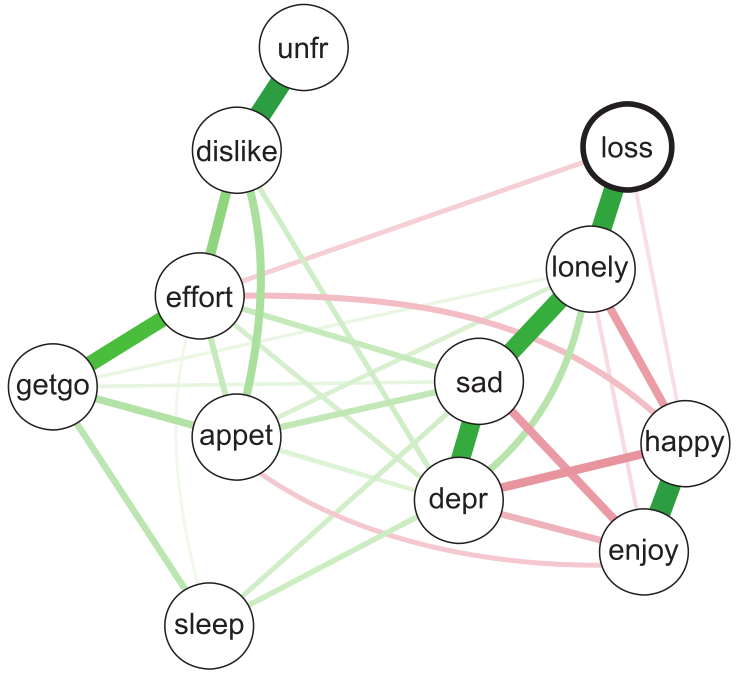
\includegraphics[width = .6 \textwidth ]{figures/psycho_network}
		\caption{Psycho-symptom network obtained from \cite{Epskamp2017}. The thickness of the line indicates the strength of the connection. Green lines indicate positive weights, red lines indicate negative weights.}
		\label{fig:network}
	\end{figure*}
	
	Although inferring the exact network of causal relations is difficult, the main point of this thesis is to show that the topological features are not predictive for the node with the highest IDT. The results from this study may provide insights in what symptoms are more dynamically important than others. This could lead to novel treatment methods for psychiatrist and psychologist alike to target symptoms that have the highest impact. Since the methods presented here do not indicate whether the impact is positive or negative for the patient, future studies will  need to validate whether these simulations contributed meaningful insights for improving the patient's quality of life. 
	
	
	\subsection{Model}\label{sec:model}
 	%discuss the details of the model, and that it is used in a
% 	variety of different fields
	Here we consider a real-signed network in which each unit is dictated by the Gibbs measure: 
	\begin{equation}
	p(s_i = x) = \frac{1}{Z(\beta)} \exp(-H(s_i))
	\end{equation}
	where $H(s_i)$ is the Hamiltonian function;
	$$H(s_i) = -\sum_{<ij>} J_{ij} s_i s_j - \sum_j h_j s_j$$
	The sum $j$ is over the nearest neighors of node $i$  
	The Gibbs measure is a concept from statistical mechanics providing a probablistic description of ensemble of particles \cite{Gibbs1996}. 
	
	\subsection{Numerical methods} \label{sec:numerical}
	In order to compute \ref{eq:mi}, we will estimate $P(x)$ and $P(x\vert X)$ using Markov chain Monte-Carlo sampling. The core procedure for a pre-defined temperature involved obtaining $N = 10 000$ snapshots based on a single Markov-Chain. Starting from a random state to eliminate, the system was equilibrated using $k = 100 000$. Next, using the state distribution, $k = 1000$ independent simulations were repeated for $\delta = 20$ time steps each to construct $p(x \vert X)$. Each simulation step consisted of asynchronous updating. Each simulation step used asynchronous updating rule; every simulation step every node in the system was considered for a flip in random order once. 
	
	Through regression with a double exponential $y = a + b\exp(-c x) + d \exp(- e x)$, we were able to estimate the decay times for each node for an $\alpha$.
	
	Previous research indicated that there is an interaction with temperature and IDT\cite{Quax2013}. Hence, in order to see the effect of noise on the symptoms we performed the procedure above for 6 temperatures. The temperatures were based on the `willingness' of the system to stay magnetized (\ref{fig:magnetizations}). Namely, the system was set to full magnetization, i.e. all nodes had state $-1$ or $+1$, and the system was ran for $N = 10 000$ steps. Temperatures were chosen between $20-80$ percent of the max magnetization (\ref{fig:magnetizations}) and as such provide a nice cross-section of the effect of noise on the system.   
	
	\begin{figure*}[ht]
		\centering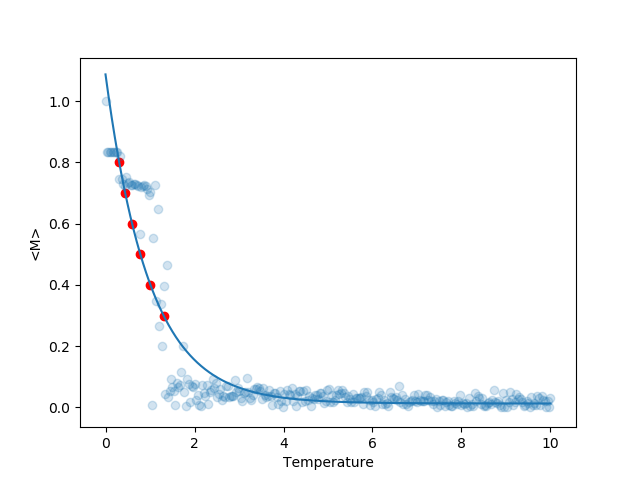
\includegraphics[width=\textwidth]{figures/magnetization-temp.png}
		\caption{Absolute magnetization as a function of temperature. The system starts from full magnetization and is simulated for 100 000 steps. The red dots indicate the magnetization between 80-20 percent of the maximum magnetization found and used for further simulations.}
		\label{fig:magnetizations}
	\end{figure*}
	
	The code used in this paper is build from the ground up in python 3.6 and can be readily adapted for use with other models, please see the appendix \ref{sec:code} for more information.
	
	\section{Results}
	
	\section{Discussion}
	% from discrete to continuous systems
	% a lot of samples needed
	\printbibliography
	\begin{appendices}
	\section{Data processing inequality}
	The data processing inequality shows that no manipulation of the data through a Markov chain can increase the inferences made from that data.
	
	Consider a Markov chain of random variables $X, Y, Z$:
	$$ X \rightarrow Y \rightarrow Z$$
	where $X \perp Z$. 

	\section{Code Manual}
	\label{sec:code}
	\section{Design philosophy}
	The main goal was to provide a package that is readily accessible and easy to adopt for use with other types of models. It is based on separation, speed, and expandability. It consists of an engine; the code used to compute the IDT and related information-theoretical measures, and methods to perform monte-carlo simulations. Other modules will hook into the engine including a model framework, basic input-output operations, see \ref{fig:code_overview} for overview.

	\section{Simple examples}
	Simple ipynb?	
	\chapter{Simple graphs}
	
	\end{appendices}
	
\end{document}
